\documentclass[a3paper,12pt]{extarticle} % Use extarticle for A3 paper size
\usepackage{graphicx} % Include this package for \includegraphics
\usepackage{amsmath}
\usepackage{amssymb} % Include this package for \mathbb
\usepackage[margin=1in]{geometry} % Adjust the margin as needed

\begin{document}

\author{kipngeno koech - bkoech}
\title{Homework 0 - Introduction to Probabilistic Graphical Models}   
\maketitle

\medskip

\maketitle

\section{Probability}
\begin{enumerate}
    \item A fair coin is tossed 10 times. The sample space for each trial is Head, Tail and the trials are independent. What is the probability of having:
    \[
        P(H) = \frac{1}{2}, \quad P(T) = \frac{1}{2}
    \]
    The probability of getting exactly \( k \) heads
    is given by the binomial distribution:
    \[
        P(X = k) = \binom{n}{k} p^k (1-p)^{n-k}
    \]
    where \( n = 10 \) and \( p = \frac{1}{2} \).
    \begin{enumerate}
        \item Zero Tail
        \[
            P(0T) = \binom{10}{0} \left(\frac{1}{2}\right)^0 \left(\frac{1}{2}\right)^{10} = \frac{1}{1024}
        \]
        \item 6 heads
        \[
            P(6H) = \binom{10}{6} \left(\frac{1}{2}\right)^6 \left(\frac{1}{2}\right)^4 = \frac{210}{1024}
        \]
        \item At least three heads
        \[
            P(X \geq 3) = 1 - P(X < 3) = 1 - P(X = 0) - P(X = 1) - P(X = 2) = 1 - \left(\frac{1}{1024} + \frac{10}{1024} + \frac{45}{1024}\right) = \frac{968}{1024}
        \]
        \item At least three Heads given the first trail was a Head!
        \[
            P(X \geq 3 | X_1 = H) = 1 - P(X < 3 | X_1 = H) = 1 - P(X = 0 | X_1 = H) - P(X = 1 | X_1 = H) - P(X = 2 | X_1 = H) = 1 - \left(\frac{1}{512} + \frac{9}{512} + \frac{36}{512}\right) = \frac{466}{512}
        \]
        \[
         = 1 - \left(\frac{1}{512} + \frac{9}{512} + \frac{36}{512}\right) = \frac{466}{512}
        \]
    \end{enumerate}
    \item Assuming the probability that it rains on Monday is 0.45; the probability that it rains on Wednesday is 0.4; and the probability that it rains on Wednesday given that rained on Monday is 0.6. What is the probability that:
    \begin{enumerate}
        \item It rains on both days
        \[
            P(M \cap W) = P(W | M)P(M) = 0.6 \times 0.45 = 0.27
        \]
        \item Rain will come next Monday, given that it has just finished raining today (Wednesday)
        \[
            P(M | W) = \frac{P(W | M)P(M)}{P(W)} = \frac{0.6 \times 0.45}{0.4} = 0.675
        \]
    \end{enumerate}
    \item Let \(X\) denote the outcome of a random experiment with possible values \{-4, -3, -2, -1, 0, 1, 2, 3, 4\} according to the following probability law:
    \[
        P(X = x) = 
    \begin{cases}
        ck^2 & \text{if } x \in \{-4, -3, -2, -1, 0, 1, 2, 3, 4\} \\
        0 & \text{otherwise}
    \end{cases}
    \]
    \begin{enumerate}
        \item What is the value of \(c\)?
        \[
            \sum_{x \in \{-4, -3, -2, -1, 0, 1, 2, 3, 4\}} P(X = x) = 1
        \]
        \[
            \sum_{x \in \{-4, -3, -2, -1, 0, 1, 2, 3, 4\}} ck^2 = 1
        \]
        \[
            c \sum_{x \in \{-4, -3, -2, -1, 0, 1, 2, 3, 4\}} k^2 = 1
        \]
        \[
            c \sum_{k = -4}^{4} k^2 = 1
        \]
        To find the value of \(c\), we can use the formula for the sum of squares of the first \(n\) natural numbers:
        \[
            \sum_{k = 1}^{n} k^2 = \frac{n(n+1)(2n+1)}{6}
        \]
        \[
            \sum_{k = -4}^{4} k^2 = \sum_{k = 1}^{4} k^2 + \sum_{k = 1}^{4} k^2 = \frac{4(4+1)(2 \times 4 + 1)}{6} + \frac{4(4+1)(2 \times 4 + 1)}{6} = 30
        \]
        \[
            c \times 30 = 1
        \]
        \[
            c = \frac{1}{30}
        \]
        \item Compute the expectation and variance of \(X\).
        \[
            E[X] = \sum_{x \in \{-4, -3, -2, -1, 0, 1, 2, 3, 4\}} xP(X = x) = \sum_{x \in \{-4, -3, -2, -1, 0, 1, 2, 3, 4\}} x \times \frac{1}{30}x^2 = \frac{1}{30} \sum_{x \in \{-4, -3, -2, -1, 0, 1, 2, 3, 4\}} x^3
        \]
        \[
            E[X] = \frac{1}{30} \sum_{x \in \{-4, -3, -2, -1, 0, 1, 2, 3, 4\}} x^3 = \frac{1}{30} \times 0 = 0
        \]
        \[
            E[X^2] = \sum_{x \in \{-4, -3, -2, -1, 0, 1, 2, 3, 4\}} x^2P(X = x) = \sum_{x \in \{-4, -3, -2, -1, 0, 1, 2, 3, 4\}} x^2 \times \frac{1}{30}x^2 = \frac{1}{30} \sum_{x \in \{-4, -3, -2, -1, 0, 1, 2, 3, 4\}} x^4
        \]
        \[
            E[X^2] = \frac{1}{30} \sum_{x \in \{-4, -3, -2, -1, 0, 1, 2, 3, 4\}} x^4 = \frac{1}{30} \times 0 = 0
        \]
        \[
            Var[X] = E[X^2] - E[X]^2 = 0 - 0 = 0
        \]
    \end{enumerate}
    \item ou just built a new COVID test with the following properties:
    \begin{itemize}
        \item If a person has COVID, the test is positive with  0.95 probability.
        \item If a person does not have COVID, the test can still be positive with 0.05 probability.
    \end{itemize}
    You are told that a random person has COVID with probability 0.001. You just use your test on a random person and it turns out to be positive. What is the probability that the person really has COVID?
    \[
        P(C) = 0.001, \quad P(\bar{C}) = 0.999
    \]
    \[
        P(T | C) = 0.95, \quad P(T | \bar{C}) = 0.05
    \]
    Bayes theorem:
    \[
        P(C | T) = \frac{P(T | C)P(C)}{P(T)}
    \]
    Probability of a positive test( Total Probability):
    \[
        P(T) = P(T | C)P(C) + P(T | \bar{C})P(\bar{C}) = 0.95 \times 0.001 + 0.05 \times 0.999 = 0.0509
    \]
    so:
    \[
        P(C | T) = \frac{0.95 \times 0.001}{0.0509} = \textbf{0.0186}
    \]
    \item You will write a python program to simulate the Monthy Hall problem. It’s a famous problem, and you can read more about it online. Suppose you’re on a game show, and you’re given the choice of three doors: Behind one door is a car; behind the others, goats. You pick a door (but don’t open it)s, say No. 1, and the host, who knows what’s behind the doors, opens another door, say No. 3, which has a goat. He then says to you, ”Do
    you want to pick door No. 2?” Is it to your advantage to switch your choice? In this simulation, the doors will be represented by an array of three elements. Each element of the
    array is either a ”0” (for the goats) or a ”1” (for the car). A python file is provided with four functions to fill.
\end{enumerate}

\newpage
\section{MLE-MAP (Warmup)}

\newpage
\section{Graph Theory}
\begin{enumerate}
    \item Degree of any Vertex of a graph is:
    \[
        \text{ (b) The number of edges incident with the vertex}
    \]
    \item In each of the following Graphs, find paths of lenght 9 and 11, and cycles of length 5, 6, 8 and 9 if possible.
    \begin{figure}[h!]
        \centering
        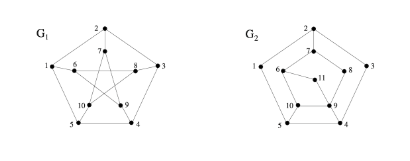
\includegraphics[width=0.8\textwidth]{PGM-graph.png}
        \caption{Graph for finding paths and cycles}
        \label{fig:pgm-graph}
    \end{figure}
    \item \begin{enumerate}
        \item 
    Find the adjacency matrix and the incidence matrix of the graph \( G = (V, E) \) where
    \( V = \{a, b, c, d, e\} \) and \( E = \{ab, ac, bc, bd, cd, ce, de\} \).

    \textbf{Adjacency Matrix:}

    \[
    A = \begin{pmatrix}
    0 & 1 & 1 & 0 & 0 \\
    1 & 0 & 1 & 1 & 0 \\
    1 & 1 & 0 & 1 & 1 \\
    0 & 1 & 1 & 0 & 1 \\
    0 & 0 & 1 & 1 & 0 \\
    \end{pmatrix}
    \]

    \textbf{Incidence Matrix:}

    \[
    I = \begin{pmatrix}
    1 & 1 & 0 & 0 & 0 & 0 & 0 \\
    1 & 0 & 1 & 1 & 0 & 0 & 0 \\
    0 & 1 & 1 & 0 & 1 & 1 & 0 \\
    0 & 0 & 0 & 1 & 1 & 0 & 1 \\
    0 & 0 & 0 & 0 & 0 & 1 & 1 \\
    \end{pmatrix}
    \]
    \item Give the adjacency list and a drawing of the graph G = ([5], E) whose adjaceny matrix:
    \[ 
    \begin{pmatrix}
        0 & 1 & 0 & 1 & 0 \\
        1 & 0 & 0 & 0 & 1 \\
        0 & 0 & 0 & 1 & 0 \\
        1 & 0 & 1 & 0 & 1 \\
        0 & 1 & 0 & 1 & 0 \\
    \end{pmatrix}
    \]
    \end{enumerate}
\end{enumerate}



\end{document}